%%
%% This is file `covers_5languages.tex',
%% generated with the docstrip utility.
%%
%% The original source files were:
%%
%% coppe.dtx  (with options: `covers')
%% 
%% This is one of the demonstration documents of the `coppe' document class:
%% the five main-language demos, the PDF/A build of the full example and the
%% side-by-side cover sheet.  It is generated from coppe.dtx by docstrip; edit
%% the .dtx source, not this file.
%% 
%% \CheckSum{0}
%% \CharacterTable
%%  {Upper-case    \A\B\C\D\E\F\G\H\I\J\K\L\M\N\O\P\Q\R\S\T\U\V\W\X\Y\Z
%%   Lower-case    \a\b\c\d\e\f\g\h\i\j\k\l\m\n\o\p\q\r\s\t\u\v\w\x\y\z
%%   Digits        \0\1\2\3\4\5\6\7\8\9
%%   Exclamation   \!     Double quote  \"     Hash (number) \#
%%   Dollar        \$     Percent       \%     Ampersand     \&
%%   Acute accent  \'     Left paren    \(     Right paren   \)
%%   Asterisk      \*     Plus          \+     Comma         \,
%%   Minus         \-     Point         \.     Solidus       \/
%%   Colon         \:     Semicolon     \;     Less than     \<
%%   Equals        \=     Greater than  \>     Question mark \?
%%   Commercial at \@     Left bracket  \[     Backslash     \\
%%   Right bracket \]     Circumflex    \^     Underscore    \_
%%   Grave accent  \`     Left brace    \{     Vertical bar  \|
%%   Right brace   \}     Tilde         \~}
%%

\documentclass[a4paper,landscape,10pt]{article}
\usepackage[margin=1cm]{geometry}
\usepackage[T1]{fontenc}
\usepackage[utf8]{inputenc}
\usepackage{graphicx}
\usepackage{caption}
\captionsetup{font=small,labelfont=bf}
\pagestyle{empty}
\begin{document}
\begin{center}
  {\Large\bfseries CoppeTeX 4.0 -- modelo multilíngue\par}
  \vspace{1mm}
  {\small As cinco línguas principais embutidas, com a mesma identidade institucional UFRJ/COPPE.\par}
\end{center}
\vspace{2mm}
\noindent
\begin{minipage}[t]{0.195\linewidth}\centering
  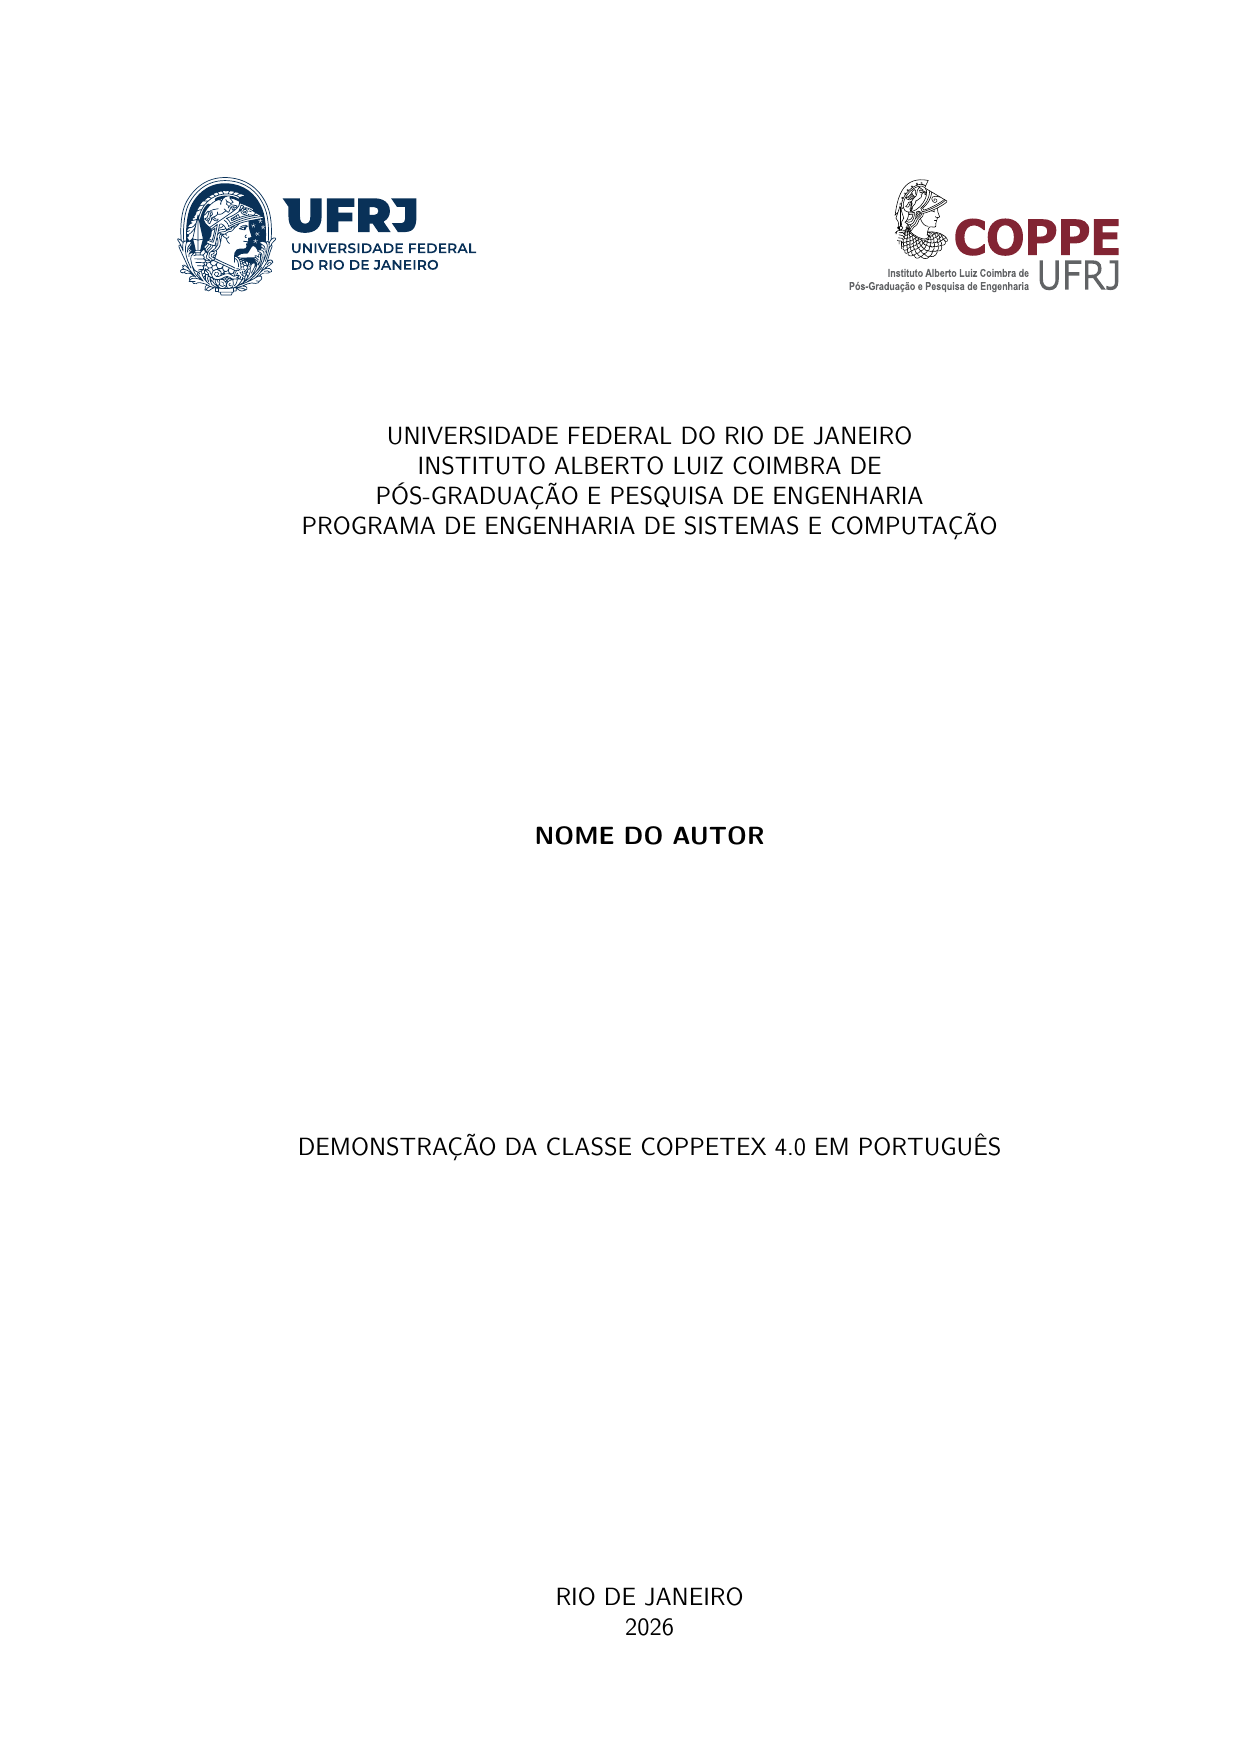
\includegraphics[width=\linewidth]{cover_pt.png}\\[1mm]
  \textbf{brazilian}\\[-0.2em]
  {\scriptsize \texttt{\textbackslash documentclass[dsc]\{coppe\}}}
\end{minipage}\hfill
\begin{minipage}[t]{0.195\linewidth}\centering
  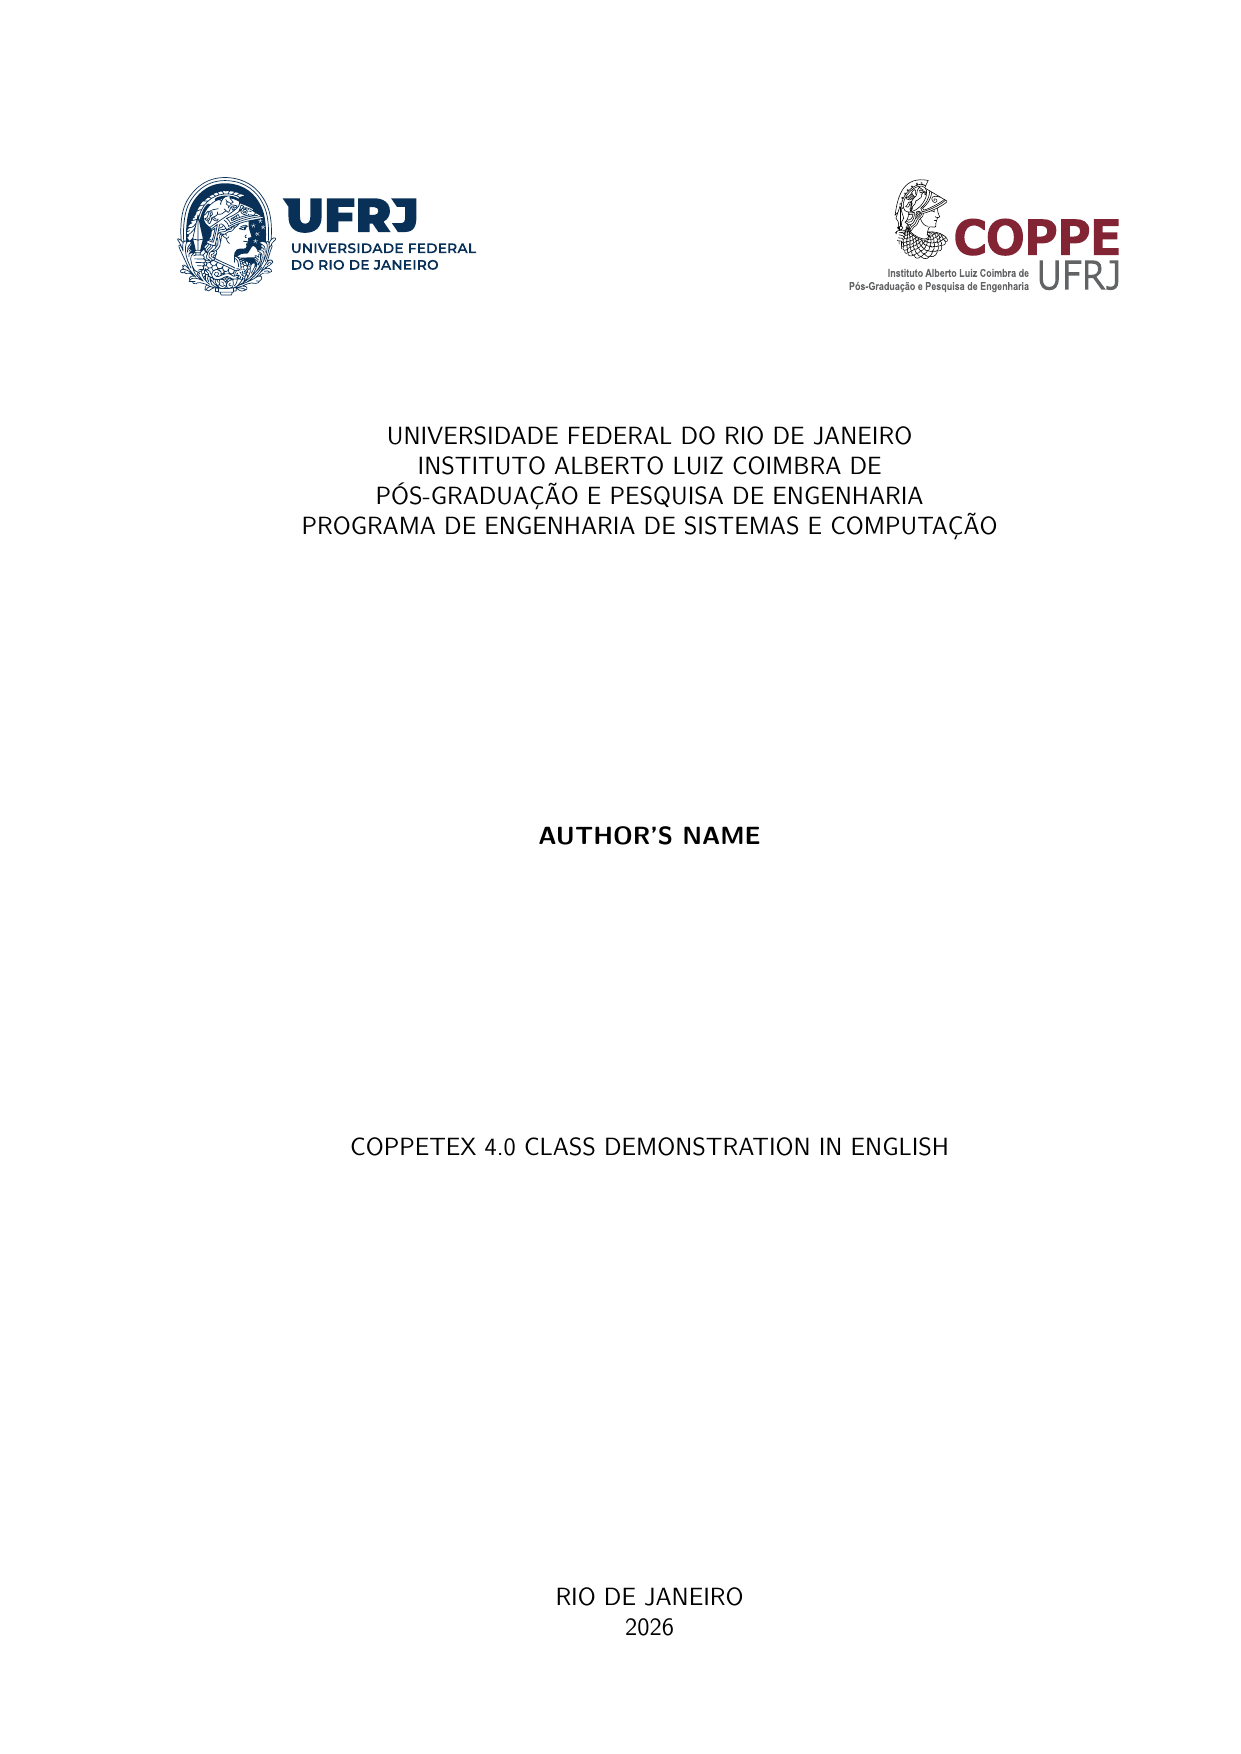
\includegraphics[width=\linewidth]{cover_en.png}\\[1mm]
  \textbf{english}\\[-0.2em]
  {\scriptsize \texttt{[english,dsc]}}
\end{minipage}\hfill
\begin{minipage}[t]{0.195\linewidth}\centering
  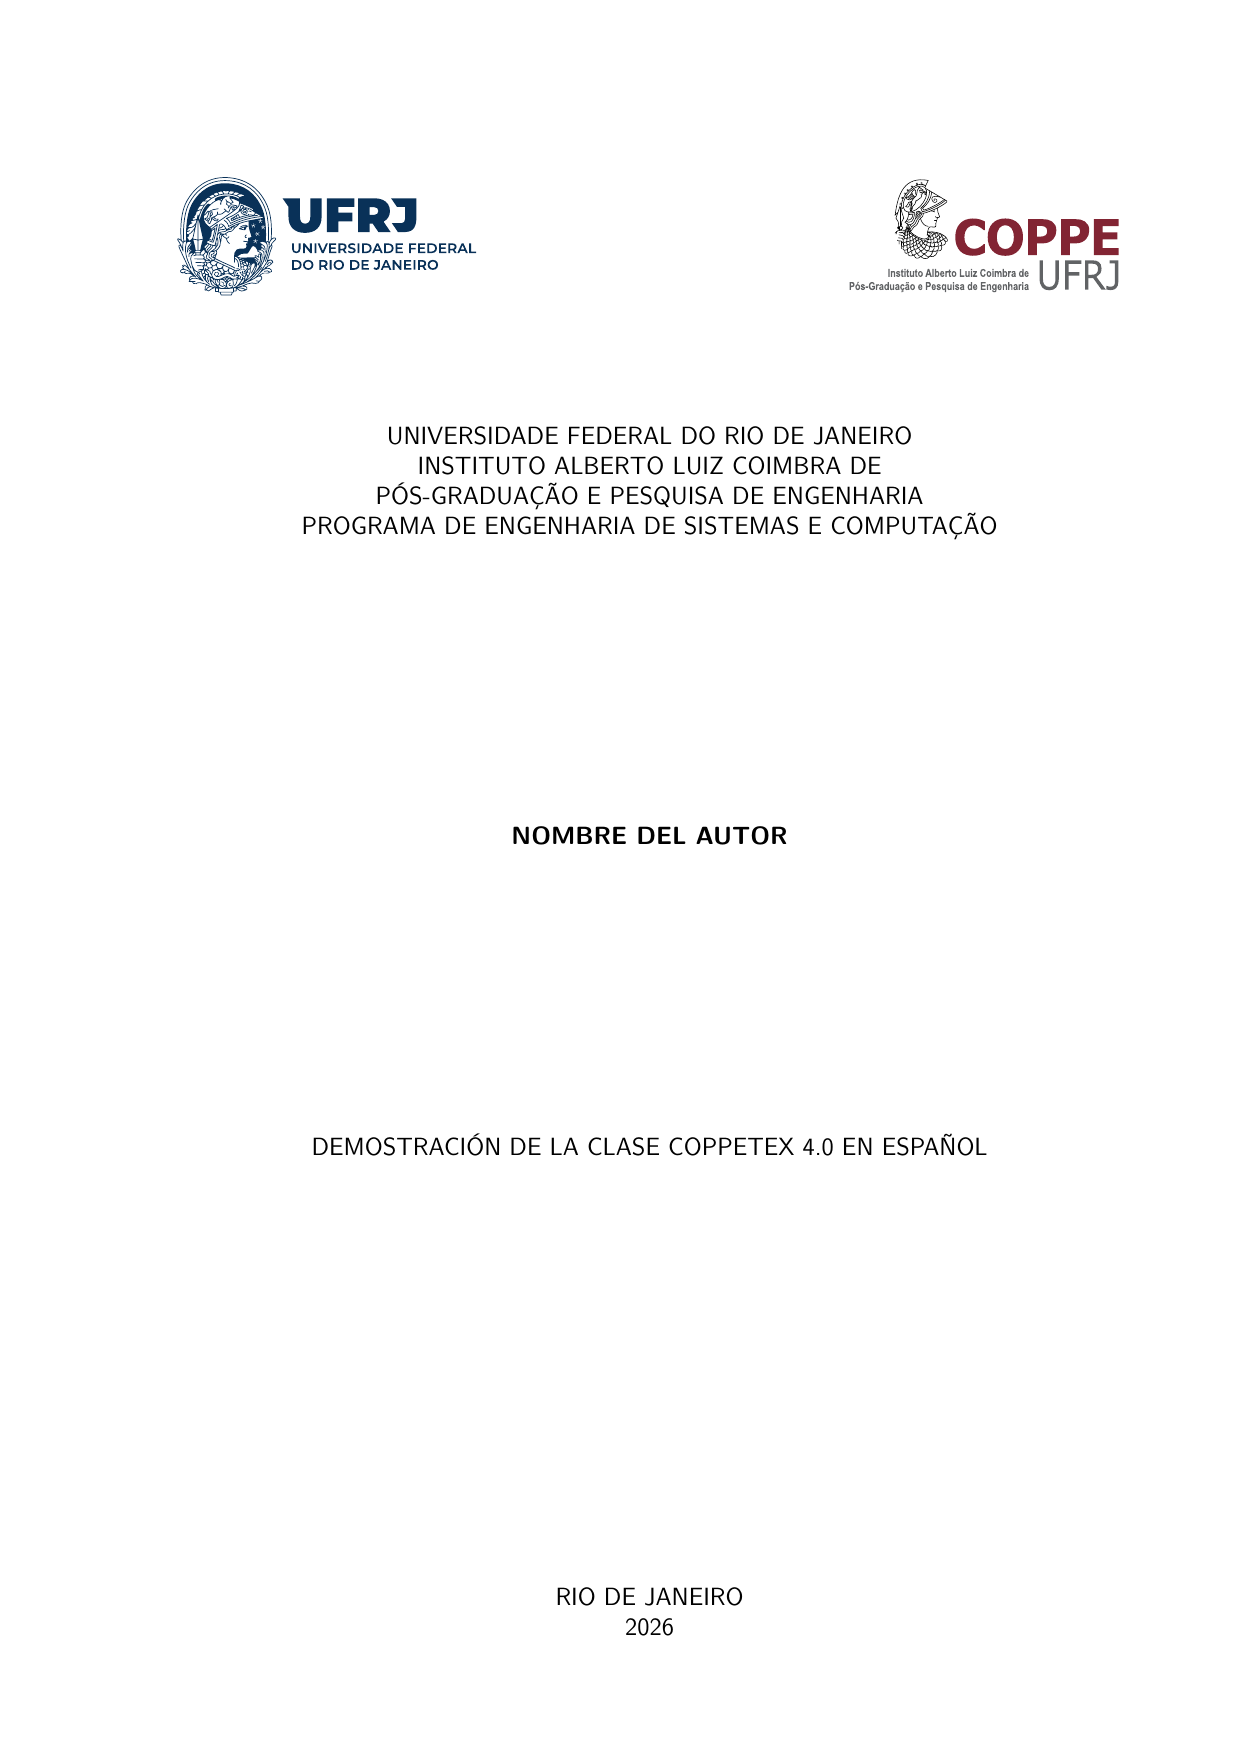
\includegraphics[width=\linewidth]{cover_es.png}\\[1mm]
  \textbf{spanish}\\[-0.2em]
  {\scriptsize \texttt{[spanish,dsc]}}
\end{minipage}\hfill
\begin{minipage}[t]{0.195\linewidth}\centering
  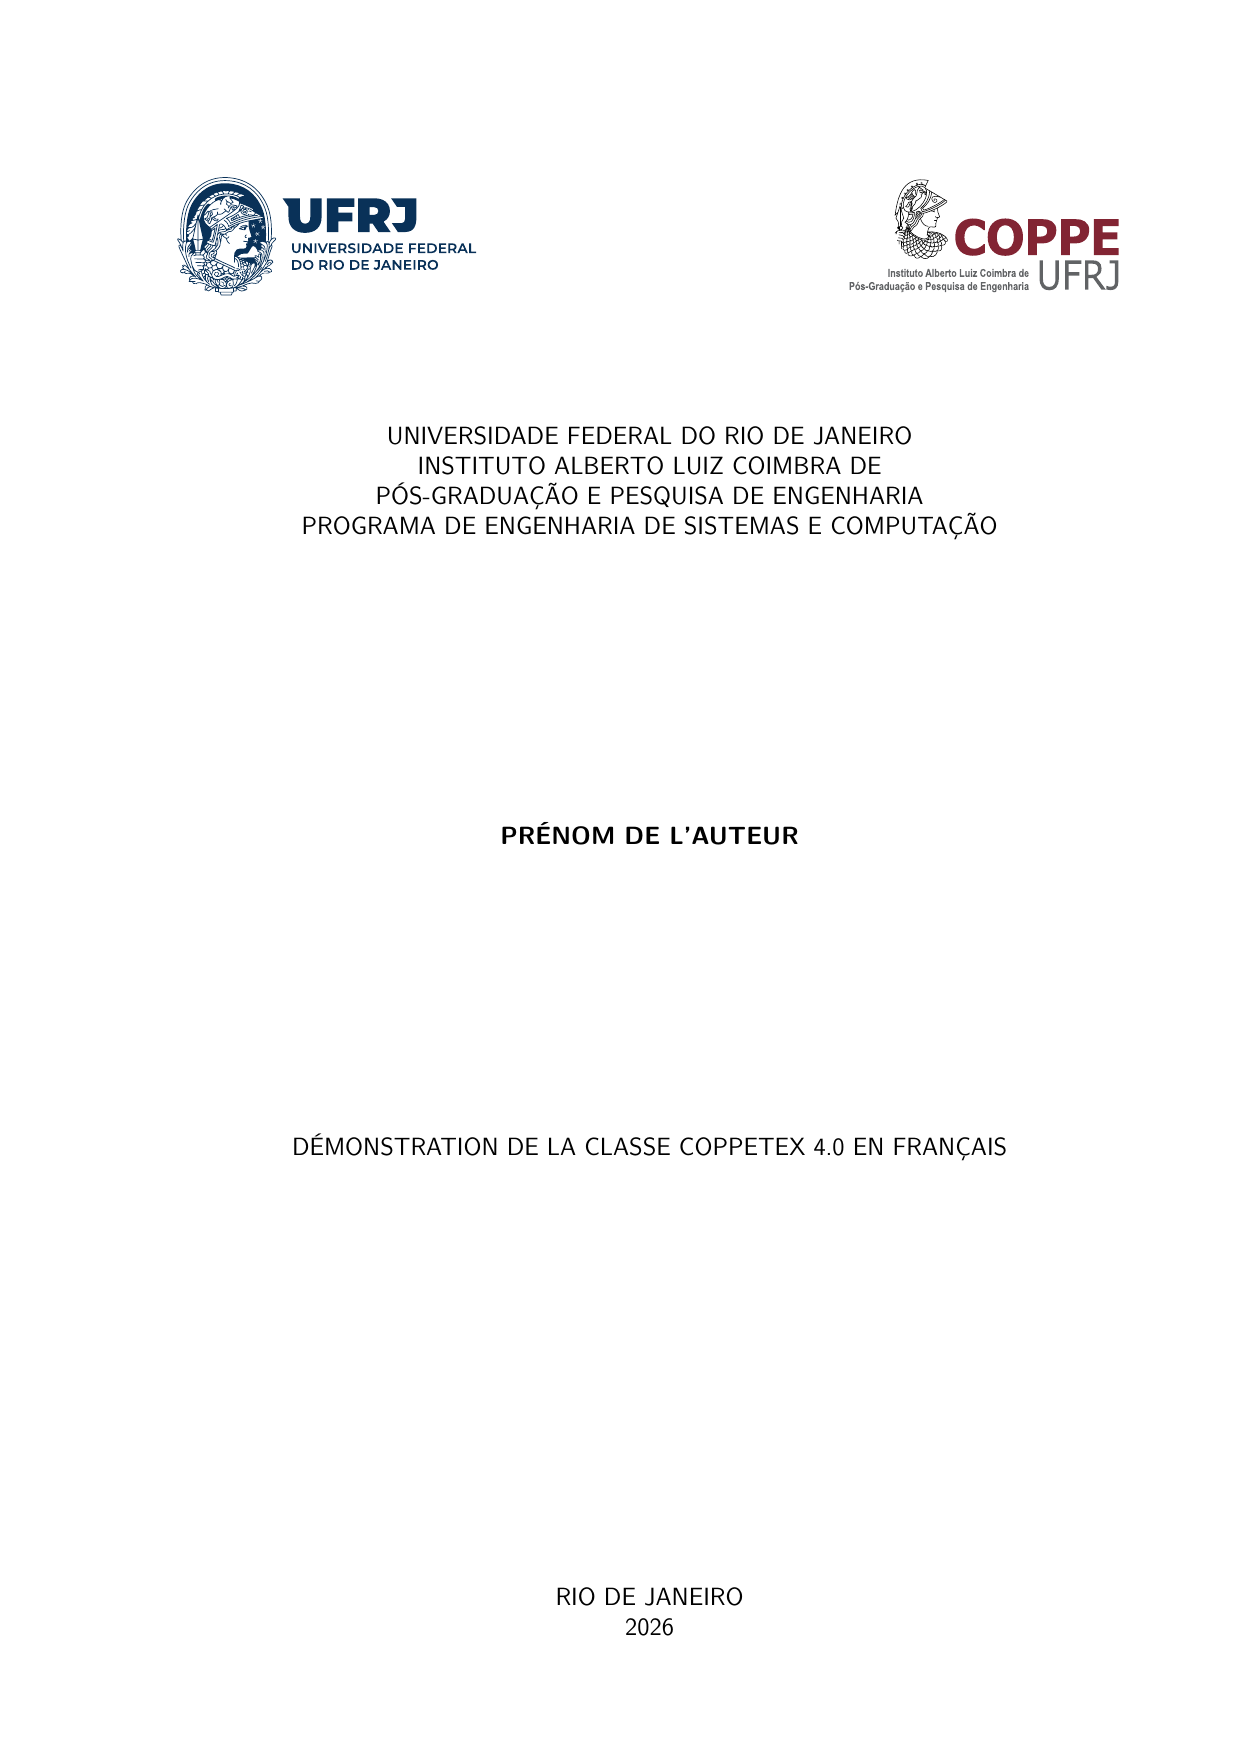
\includegraphics[width=\linewidth]{cover_fr.png}\\[1mm]
  \textbf{french}\\[-0.2em]
  {\scriptsize \texttt{[french,dsc]}}
\end{minipage}\hfill
\begin{minipage}[t]{0.195\linewidth}\centering
  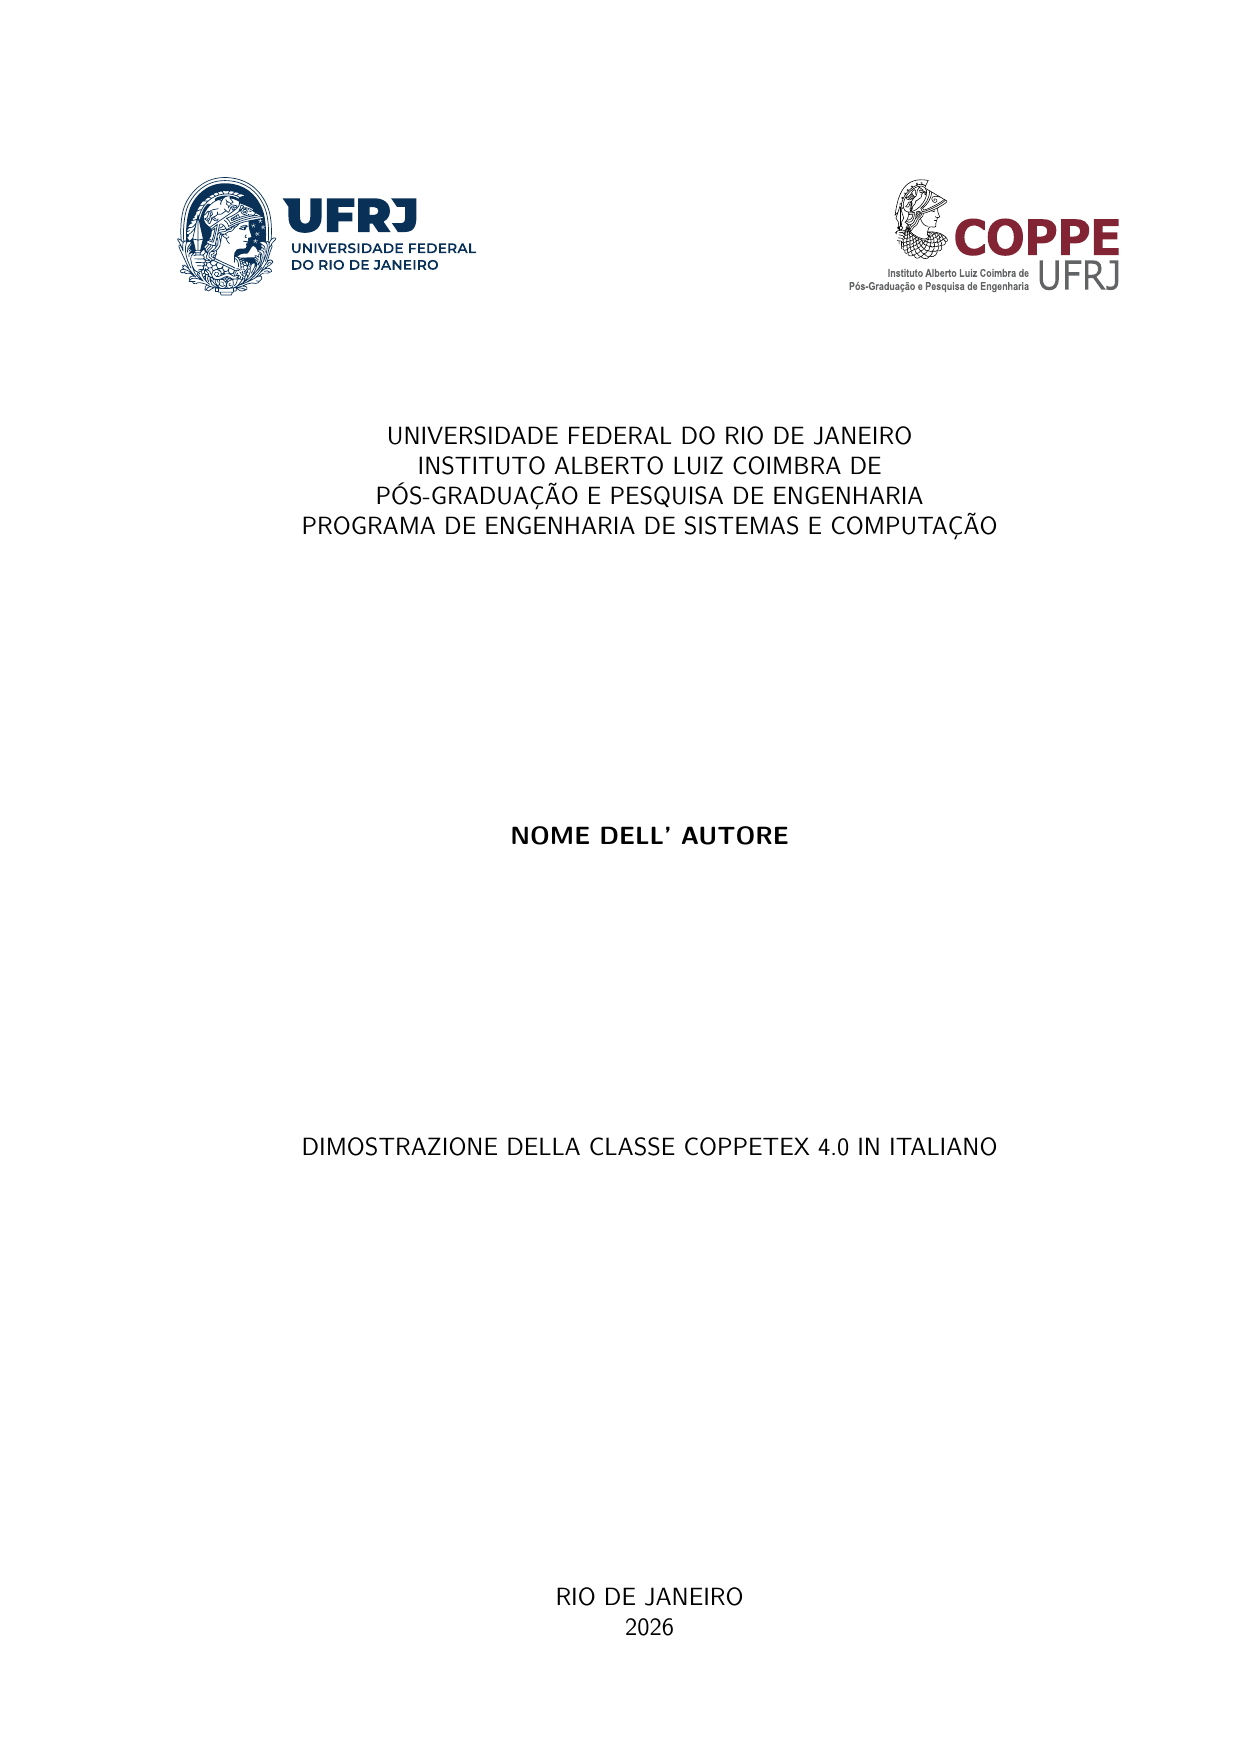
\includegraphics[width=\linewidth]{cover_it.png}\\[1mm]
  \textbf{italian}\\[-0.2em]
  {\scriptsize \texttt{[italian,dsc]}}
\end{minipage}

\vfill
\noindent\footnotesize
\textbf{Observe que:} (1) o bloco institucional no topo
(\emph{Universidade Federal do Rio de Janeiro}, \emph{Instituto Alberto
Luiz Coimbra de Pós-Graduação e Pesquisa de Engenharia (COPPE)},
\emph{Programa de Engenharia de Sistemas e Computação}) permanece em
português em todas as capas, por se tratar de identidade institucional
da UFRJ;
(2) o título do trabalho acompanha o idioma principal escolhido na opção
da classe;
(3) a cidade e o ano no rodapé também ficam em português.

\hfill\textit{Imagens geradas a partir dos arquivos \texttt{example\_\{pt,en,es,fr,it\}.tex} em \texttt{dist/}.}
\end{document}
%% 
%%
%% End of file `covers_5languages.tex'.
